%!TEX root = ../../../adrien_gomar_phd.tex

\paragraph{Using the advection equation model problem}

A pure harmonic signal is imposed at the left boundary condition
of the advection equation model problem:
\begin{equation}
   u_l (t) = 1 + a \sin \left(2 \pi f t\right).
\end{equation}
The time instances of the harmonic balance
computations are chosen to reach varying condition numbers
such that $1 \leq \kappa (E) \leq 1.1$.  
The minimal conditioning
$\kappa(E) = 1$ is obtained with evenly spaced time instances.

By definition, the condition number amplifies the error 
on the iterative resolution of the advection equation.
This is illustrated in Fig.~\ref{fig:condition_number_local_amp} which 
shows the evolution of the results with a varying condition number.
The amplitude of the
sinusoidal function is either under or over-estimated. However, 
the higher the condition number, the worse the accuracy in capturing
the amplitude of the injected function.
\begin{figure}[htbp]
  \centering
  \includegraphics*[width=0.40\textwidth]{condition_number_local_amp.pdf}
  \caption{Linear advection of a sinusoidal function: numerical steady-state 
  solutions at $t=0$ for varying condition number.}
  \label{fig:condition_number_local_amp}
\end{figure}

To have a more quantitative insight of the issue raised by a 
growing condition number, the evolution of the
$\mathcal{L}2$-norm of the error as a function of the condition
number and the amplitude is shown in Fig.~\ref{fig:condition_number}.
The amplitude of the unsteadinesses varies between: $0.1 \leq a \leq 1$.
Ten points are used to sample the amplitude and condition number intervals
which gives 100 computations in total.
Clearly, the error increases
when the condition number and the amplitude of the
unsteadinesses grow. This was expected as the condition
number, by definition, sets an upper bound of
the error made by iteratively resolving the advection equation
as defined in Eq.~\eqref{eq:conditonnig_amp}.
\begin{figure}[htb]
  \centering
  \includegraphics*[width=0.40\textwidth]{condition_number.pdf}
  \caption{$\mathcal{L}2$-norm of the error as a function of the condition number
  $\kappa(E)$ and the amplitude of the injected unsteadinesses.}
  \label{fig:condition_number}
\end{figure}


\paragraph{Using the channel flow toy problem}
The previous example was based on the advection equation which
has the good property of having a analytical solution to 
analyze the results. The results show that the harmonic
balance solutions are very sensitive to the condition number.
To further analyze the condition number issue,
the unsteady channel flow toy problem
(see Sec.~\ref{sec:toy_channel}) is computed with a single
frequency oscillating back-pressure 
at the outlet: $f_1 = 3$~Hz, the second
frequency having a zero amplitude: $a_2= 0$:
\begin{equation}
   P_{outlet} (t) = P_m \left[ 1 + a_1 \sin \left(2 \pi f_1 t\right) \right].
\end{equation}
This helps understanding the behavior of the HB source term
coupled to the Navier--Stokes equations.
Therefore, the oscillating back-pressure is mono-frequential.
By using evenly-space time instances, the condition
number of the source term is unity $\kappa (E) = 1$. 
Thus, to highlight the issue related to the condition number,
the time instances are chosen to reach varying condition numbers
such that $1 \leq \kappa (E) \leq 3.43$.  

Two frequencies are
specified for the HB computation: $f_1$ and its first harmonic
$2f_1$.
As shown above, the condition number amplifies numerical errors and that these
depends on the unsteady phenomenon computed, it is chosen to
test two amplitudes for the oscillating back-pressure: $a_1 = 0.05$
and $a_1=0.01$.

\begin{figure}[htb]
  \centering 
  \subfigure[$a_1=0.01$]{
    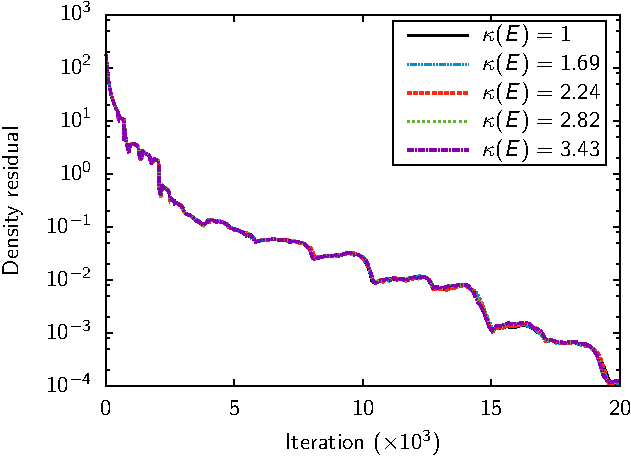
\includegraphics[width=.45\textwidth]{CANAL2_RESIDUAL_VS_CONDITIONNING_AMP001_PPT.pdf}}
  \subfigure[$a_1=0.05$]{
    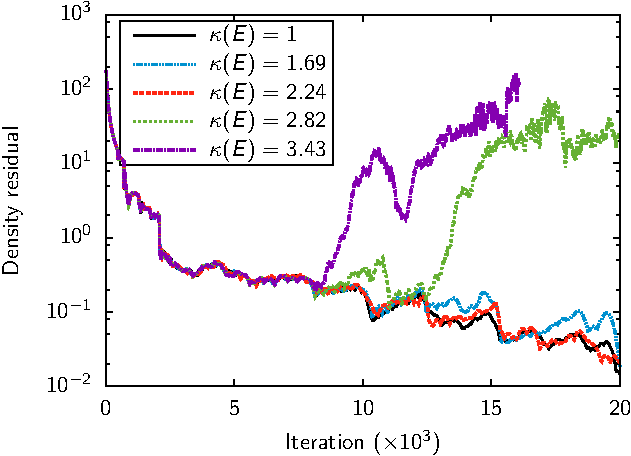
\includegraphics[width=.45\textwidth]{CANAL2_RESIDUAL_VS_CONDITIONNING_AMP005_PPT.pdf}}
  \caption{Relation between the condition number $\kappa (E)$ and the
    convergence of the solution.}
  \label{fig:canal_residual_vs_conditionning}
\end{figure}
The convergence of the computations with varying condition number 
$1 \leq \kappa (E) \leq 3.43$ and
amplitudes is shown as the evolution of the density residual in 
Fig.~\ref{fig:canal_residual_vs_conditionning}.
For a condition number $\kappa (E) \geq 3.43$ and wave input amplitude
$a_1 = 0.05$, the computation diverges. However, the computations with
the same condition numbers but a smaller input amplitude $a_1 = 0.01$
converge. In fact, the condition number amplifies the errors made
during the iterative process. When the input waves have a smaller
amplitude, the iterative errors are slighter, hence the convergence as
explained Sec.~\ref{sec:sm_hb_multi}.

\todo[inline, color=yellow]{local results to show if solution is OK}